\documentclass{article}

\usepackage{graphicx}

\begin{document}



\title{Project Document}



\maketitle



\section{Kata Pengantar}

Dokumen ini memberikan kata - kata untuk hasil skripsi anda bro



% Menggunakan \MakeLinkTarget untuk membuat tautan

\MakeLinkTarget{youtube-video}{https://www.youtube.com/watch?v=dQw4w9WgXcQ}







\section{Pendahuluan}

Ini adalah bagian pendahuluan dari dokumen Anda. Ini adalah keren

\section{Tinjauan Pustaka}

Di sini Anda dapat menulis tinjauan pustaka yang relevan dengan topik.









\section{Hasil dan Pembahasan}

Sajikan hasil analisis Anda dan bahas temuan yang relevan. 

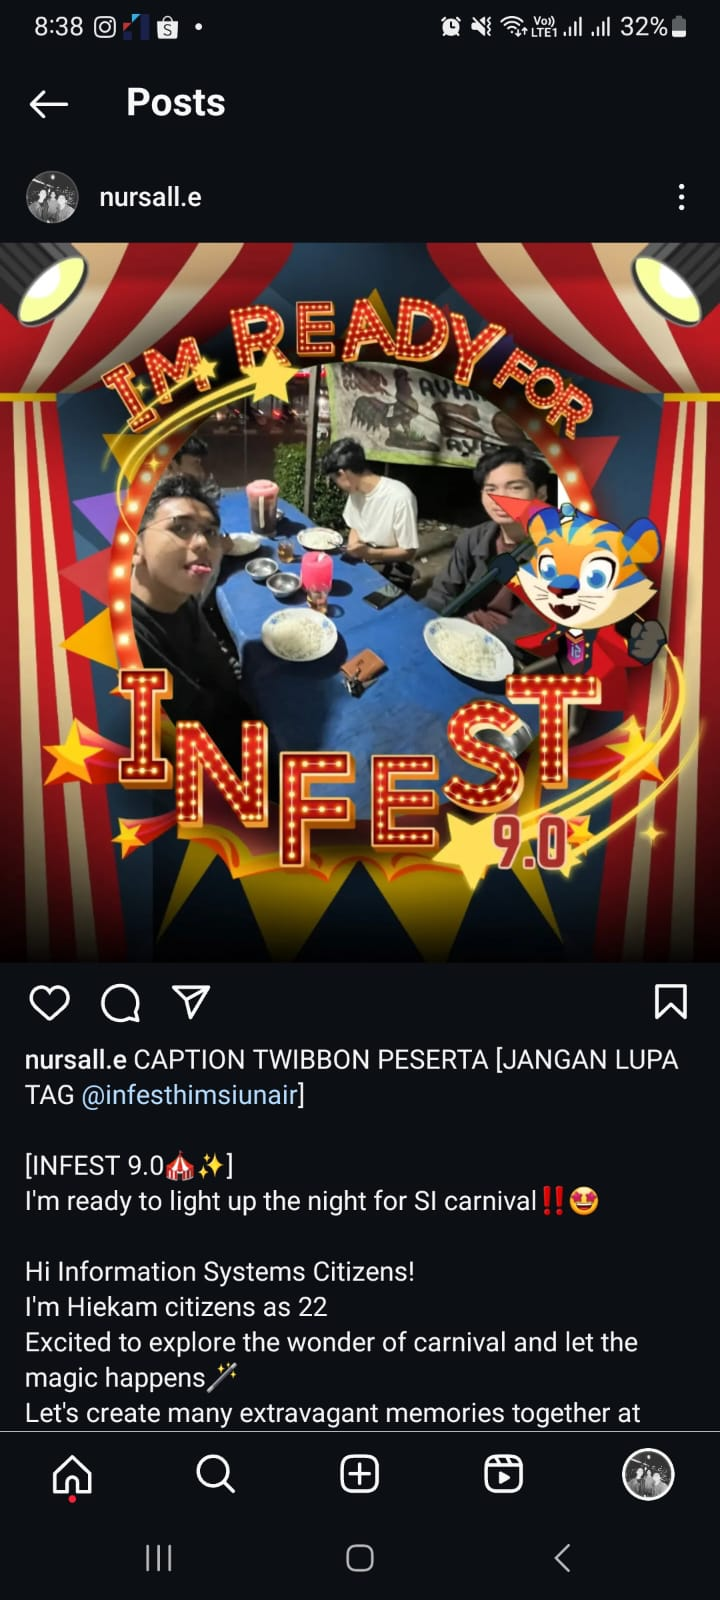
\includegraphics[width=0.8\textwidth]{images/1_20241102151715.jpg} % Sesuaikan ukuran



asdhahsd

\section{Kesimpulan}

Simpulkan temuan dan rekomendasi dari penelitian atau analisis Anda.



% Tautan ke YouTube

\textbf{Tautan Video YouTube:https://www.youtube.com/watch?v=dQw4w9WgXcQ} \hyperlink{https://www.youtube.com/watch?v=dQw4w9WgXcQ}{Klik di sini untuk menonton video!}

\end{document}